
\section{Experiments}

Once we have implemented all these tables, we can start by comparing their relative performances. We have therefore set up a simple experimental protocol to test the different properties and actions that interest us. Here, we focused on three types of possible actions, inserting a new element, obtaining a value and searching for an element not present in the table. Deletion operations were not considered due to the excessive analogy of the processing carried out in relation to search operations. We then ran all the experiments in the same framework, 32 warps and 32 blocks, all threads doing the same operation on different data. Finally, we took the statistics related to the execution of 30 runs and this on 10 iterations. We decided to perform the experiments under a load factor of 50\%, it implies that we preallocate enough memory to hold twice our data, and for a number of operations between 65 thousands $(2^{15})$ up to 8 millions $(2^{23})$. We will represent the mean obtained with the standard deviation as a dot in the following.

\subsection{Insertion}

We will start by presenting the results obtained for the insertions:

\begin{figure}[!ht]
\centering
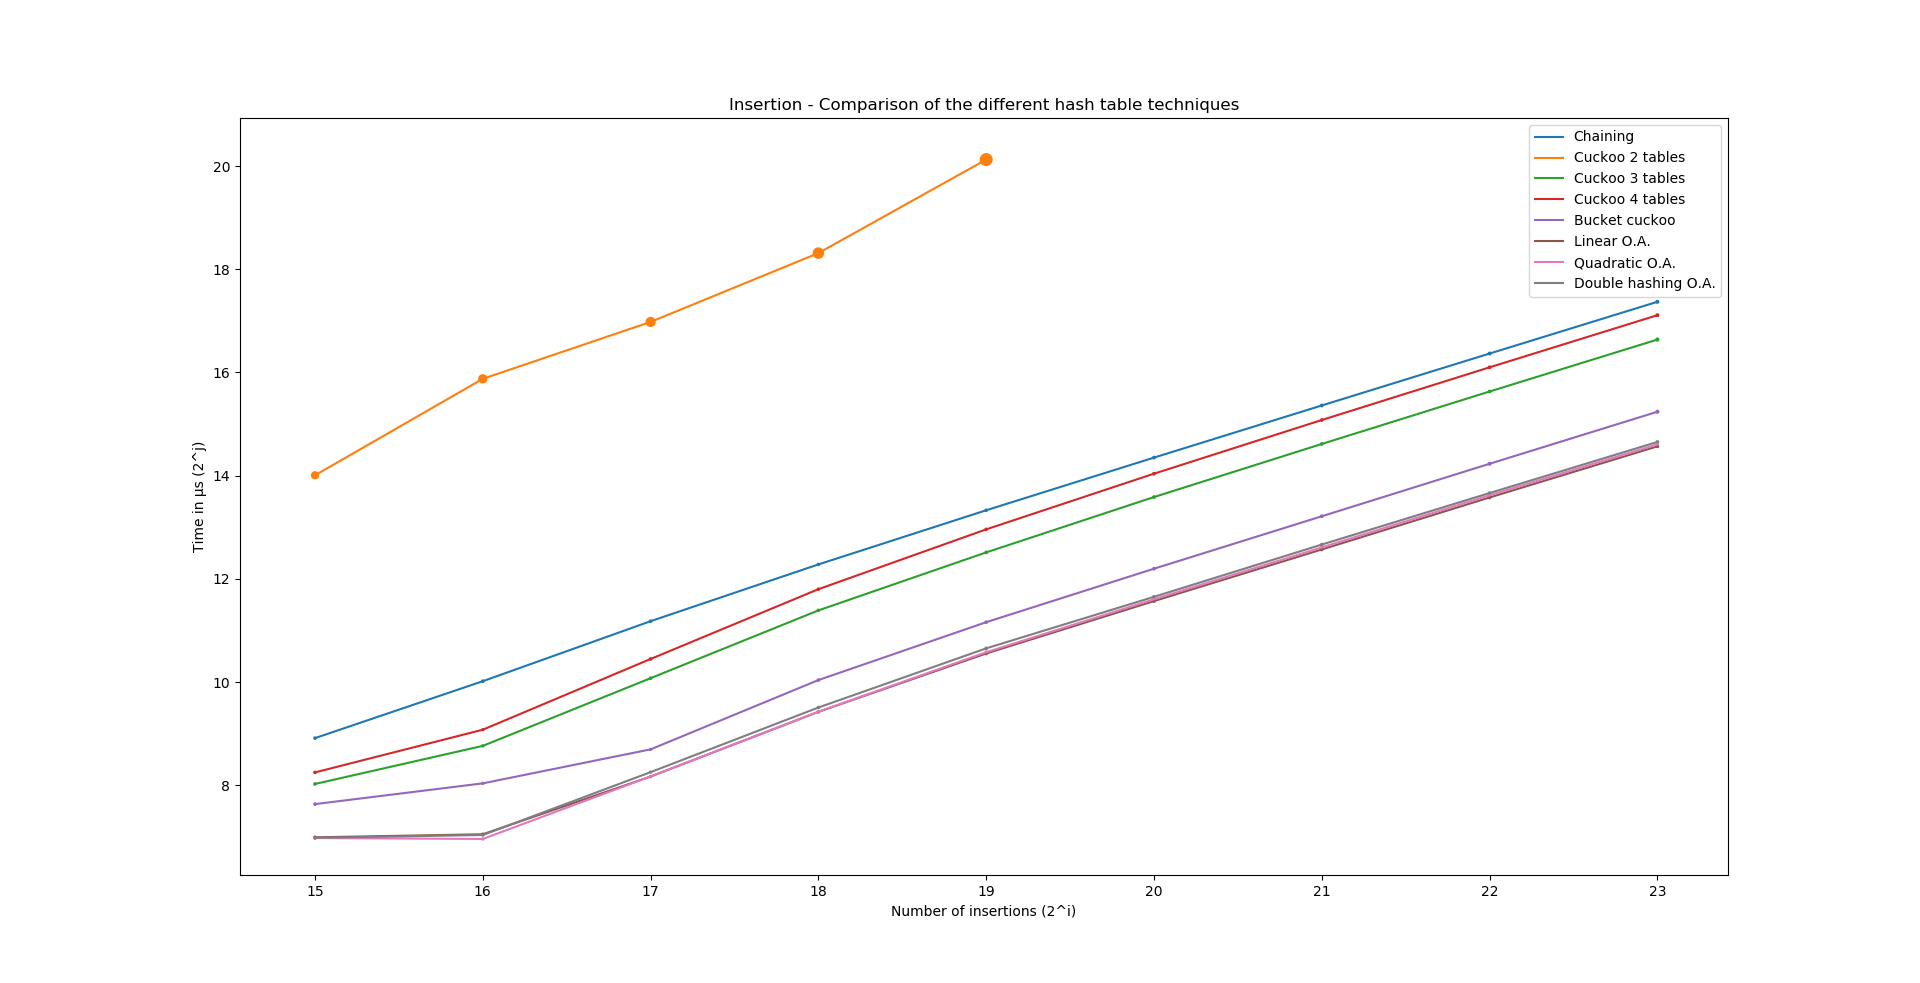
\includegraphics[width=\linewidth]{Chapters/HashTable/Results/DictionaryInsertions.png} 
\caption{Insertions in hash table\index{Hash table} 32-bit key/value}
\end{figure}

Different results can be seen on these graphs:

\begin{itemize}
    \item Cuckoo\index{Cuckoo hashing} hashing with two tables seems to present catastrophic results compared to other models. We also decided to stop its experiment after having exceeded the million of insertions seen the time necessary for the action (attention to the log plot). A very important remark must be made a priori, we present here the mean, but the median is in reality only 1.34 times larger than for the insertion with cuckoo\index{Cuckoo hashing} and 3 tables, it should lie in reality somewhere between 3 and 4 tables. This also implies that one can fall in strongly degenerated cases where the active waiting leads to much contention, which makes explode the execution time.
    \item The very essence of cuckoo\index{Cuckoo hashing} operation leads to a much stronger sequentiality\index{Sequential} of actions, and as one may be led to transfer many table elements to table, this induces very strong adverse cases. A more adapted tuning of the parameters as well on the level of the size of the tables as in the functions of hashage employed can partially mitigate these problems.
    \item Chaining\index{Chaining} proposes surprisingly low performances which can be explained by the mode of access to the data and the indirection necessary to access the data, one has a low efficiency in the use of the cache\index{Cache}.
    \item We can also note that the cuckoo\index{Cuckoo hashing} with more than 2 tables and buckets of size 4 leads to a noticeable acceleration of performance. So, once a cached line\index{Block} has been loaded, its access becomes essentially free.
    \item Finally, those who use notions related to open addressing\index{Open addressing} fare best. They even fit in a pocket handkerchief; no noticeable difference, mainly due to the relatively low load factor, 50\%.
\end{itemize}

\subsection{Search}

We can then move on to the two search operations, one successful and the other looking for an element that does not exist:

\begin{figure}[!ht]
\centering
  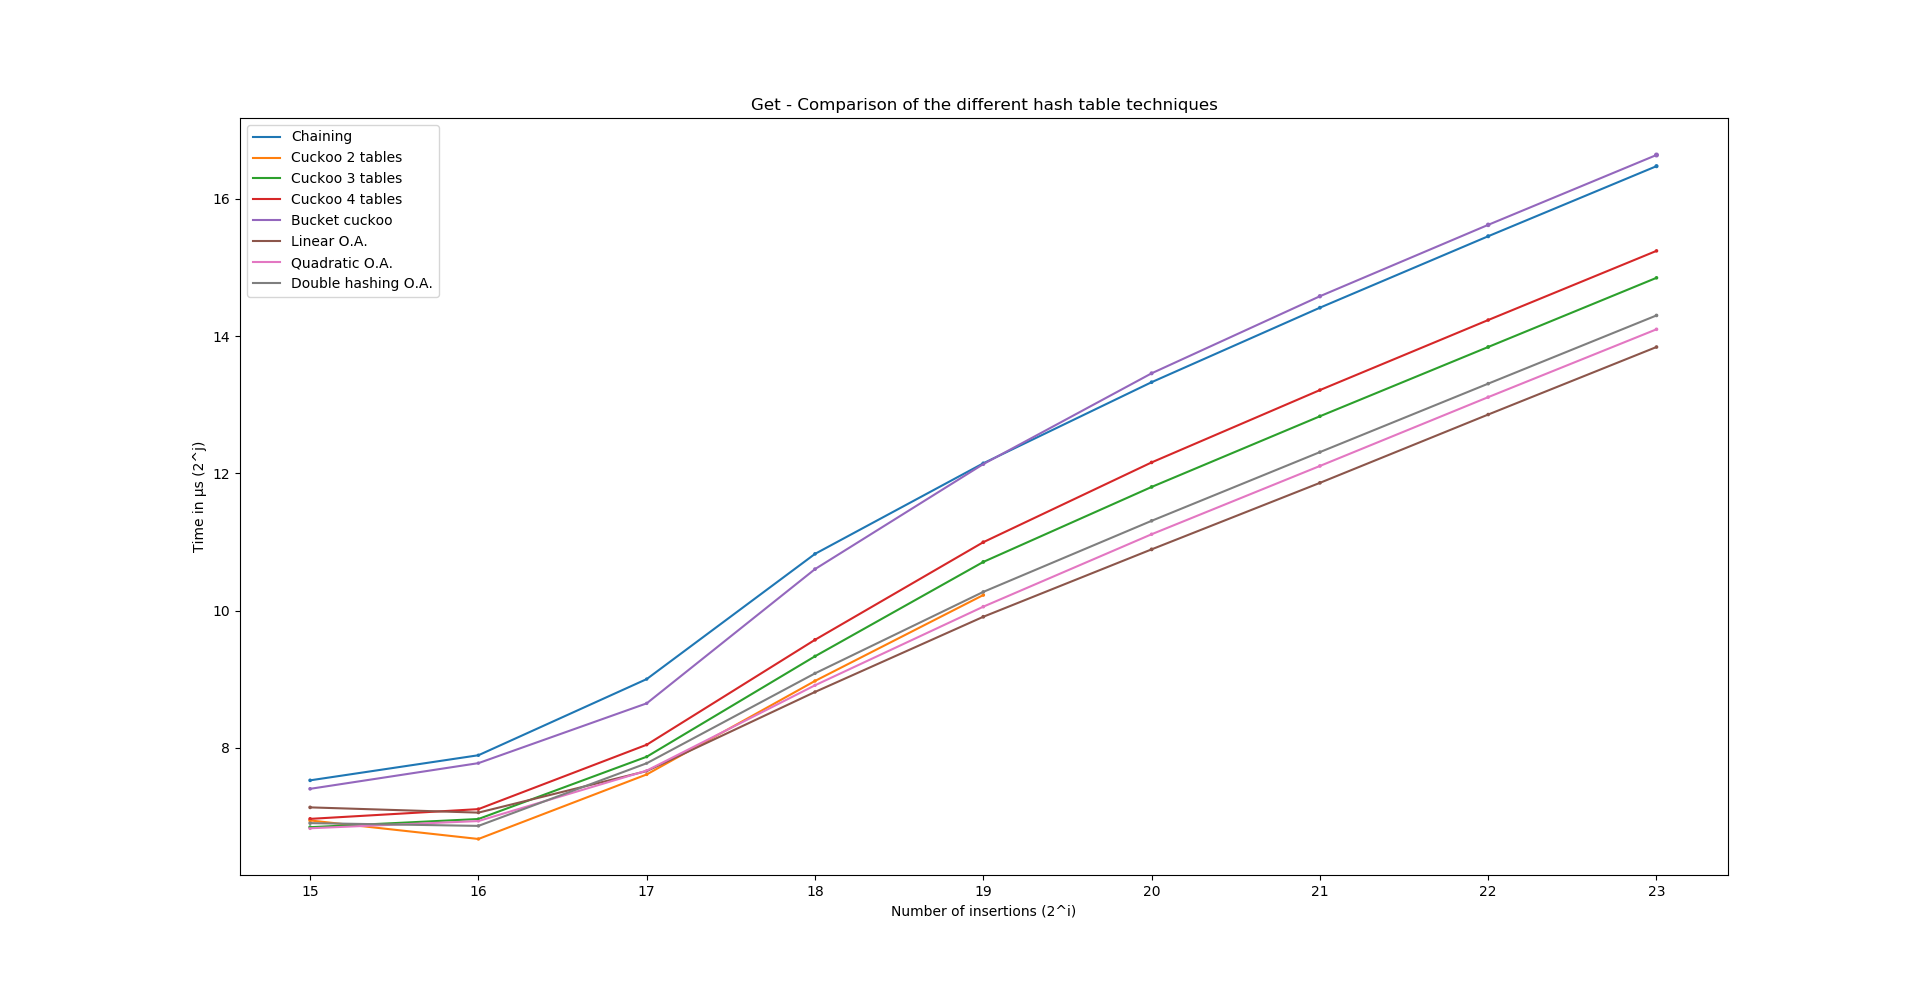
\includegraphics[width=\linewidth]{Chapters/HashTable/Results/DictionaryGet.png}
  \captionof{figure}{Successful search}
  \label{fig:successful_get}
 \end{figure}
 
\begin{figure}[!ht]
  \centering
  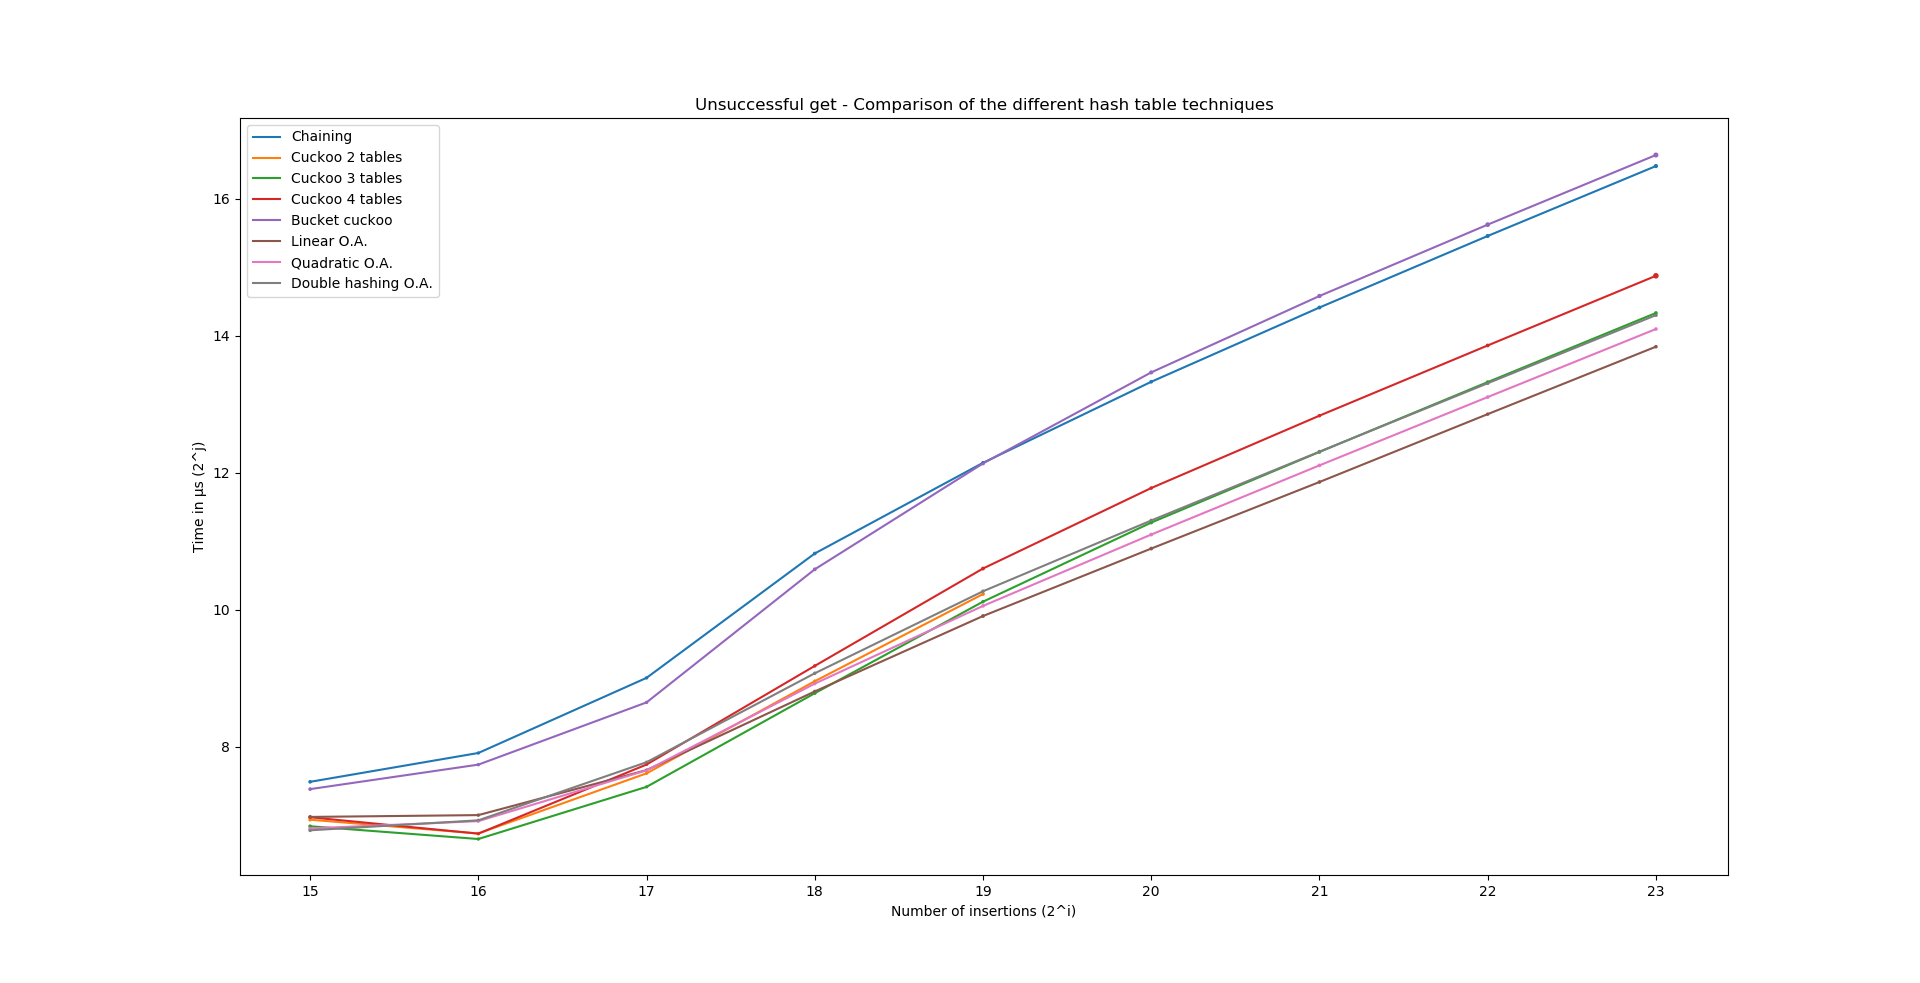
\includegraphics[width=\linewidth]{Chapters/HashTable/Results/DictionaryGetUnsuccessful.png}
  \captionof{figure}{Unsuccessful search}
  \label{fig:unsuccessful_get}
\end{figure}

Again, many remarks to be made:
\begin{itemize}
    \item Chaining\index{Chaining} and cuckoo\index{Cuckoo hashing} with bucket present the worst results of all these techniques. The performance is quite logical since these techniques are based on a similar scheme where all elements associated with a value must be observed before moving to the next node/table. A lot of processing is then done and the divergence in the same warp is all the greater as the number of possible branching may exist.
    \item When there are few elements, cuckoo hashing\index{Cuckoo hashing} seems to offer a real alternative to open addressing\index{Open addressing} with a lower standard deviation and a slightly lower but still significant average (by unpaired t-test). But on a larger number the interest seems tenuous. Indeed, the locality of the data and their relative efficiency play a crucial role in access times. Accessing the entire cache line\index{Block} even if loaded randomly and concurrently by each thread remains comparable to lower efficiency but with sequential\index{Sequential} accesses.
    \item A notable and curious difference exists between the two cases of searches. If the element exists, cuckoo\index{Cuckoo hashing} with 2 tables shows the best access times. On the contrary, if the element is absent, 3 tables seem slightly more effective. This phenomenon is somewhat bizarre and difficult to explain. It seems logical that searching in fewer tables takes less time since you have to load less data in the end but the other case is a real mystery.
    \item Finally, a linear probing\index{Probing} seems to be the best in our case (50\% of load factors), we then find quite naturally quadratic and double hashing since quadratic offers at the beginning, a greater probability to remain in the same cache line\index{Block}, whereas with double hashing, it becomes practically nil. It is funny to note that cuckoo hashing\index{Cuckoo hashing} and double hashing seem to offer the same performance, which would indicate that an equivalent number of data are read in both cases, i.e. 2.
\end{itemize}

\subsection{Conclusions}

Cuckoo hashing\index{Cuckoo hashing} with just two tables is not a viable alternative in the context of graphics cards\index{Graphics cards}. Unless the static insertion approach is chosen as originally presented~\cite{alcantara2009real}. Working with 3 tables (at least) or with buckets seems a much better alternative but buckets have the disadvantage of having relatively slow access times to the elements and, in the end, one would prefer to use 3 tables if the cuckoo\index{Cuckoo hashing} approach is really necessary. This has the advantage of having a bounded time on search operations compared to the other two families and the standard deviation is slightly lower, which is better suited to real time conditions. It is also the technique that can afford a high load factor without paying too much on the resulting performances.

Chaining\index{Chaining} does not seem to offer any interest by itself, if we obviously omit the possibilities of resizing the data structure and its flexibility in memory. It is much easier to offer strong guarantees on the validity of operators in this context.

Open addressing\index{Open addressing} seems to be the big winner of our test, both in terms of insertions and searches. However, the removal policy is a little more complex and it may be necessary to clean this table regularly, which induces a cost in fine. Hopscotch hashing~\cite{herlihy2008hopscotch} presents a very interesting variant to these techniques since it consists in limiting the region in which an element can be located by exchanging the position of two elements as long as they remain sufficiently close to their original position. This would introduce a cost on insertions but would help reduce the worst case in search operations. Moreover, the linear variant of open addressing\index{Open addressing} seems to win hands down in each of the tested conditions, we will opt for it when implementing our X-fast trie\index{X-fast trie}.

Finally, the results are more or less the same using 64-bit keys, but there is a greater decrease in performance for linear open addressing\index{Open addressing} than in any other case due to the greater number of memory requests made. But the latter remains a winner in all cases. Finally, in order to give perspectives on the possible performances obtained, our implementation allows the insertion of 325 million elements per second and to recover the value associated with 572 million keys per second. See also, Heer et al.~\cite{heerdata} which regroup all the results obtained for hash tables\index{Hash table} on GPU\index{Graphics cards}.
